% Options for packages loaded elsewhere
\PassOptionsToPackage{unicode}{hyperref}
\PassOptionsToPackage{hyphens}{url}
\PassOptionsToPackage{dvipsnames,svgnames,x11names}{xcolor}
%
\documentclass[
  letterpaper,
  DIV=11,
  numbers=noendperiod]{scrreprt}

\usepackage{amsmath,amssymb}
\usepackage{iftex}
\ifPDFTeX
  \usepackage[T1]{fontenc}
  \usepackage[utf8]{inputenc}
  \usepackage{textcomp} % provide euro and other symbols
\else % if luatex or xetex
  \usepackage{unicode-math}
  \defaultfontfeatures{Scale=MatchLowercase}
  \defaultfontfeatures[\rmfamily]{Ligatures=TeX,Scale=1}
\fi
\usepackage{lmodern}
\ifPDFTeX\else  
    % xetex/luatex font selection
\fi
% Use upquote if available, for straight quotes in verbatim environments
\IfFileExists{upquote.sty}{\usepackage{upquote}}{}
\IfFileExists{microtype.sty}{% use microtype if available
  \usepackage[]{microtype}
  \UseMicrotypeSet[protrusion]{basicmath} % disable protrusion for tt fonts
}{}
\makeatletter
\@ifundefined{KOMAClassName}{% if non-KOMA class
  \IfFileExists{parskip.sty}{%
    \usepackage{parskip}
  }{% else
    \setlength{\parindent}{0pt}
    \setlength{\parskip}{6pt plus 2pt minus 1pt}}
}{% if KOMA class
  \KOMAoptions{parskip=half}}
\makeatother
\usepackage{xcolor}
\setlength{\emergencystretch}{3em} % prevent overfull lines
\setcounter{secnumdepth}{5}
% Make \paragraph and \subparagraph free-standing
\ifx\paragraph\undefined\else
  \let\oldparagraph\paragraph
  \renewcommand{\paragraph}[1]{\oldparagraph{#1}\mbox{}}
\fi
\ifx\subparagraph\undefined\else
  \let\oldsubparagraph\subparagraph
  \renewcommand{\subparagraph}[1]{\oldsubparagraph{#1}\mbox{}}
\fi

\usepackage{color}
\usepackage{fancyvrb}
\newcommand{\VerbBar}{|}
\newcommand{\VERB}{\Verb[commandchars=\\\{\}]}
\DefineVerbatimEnvironment{Highlighting}{Verbatim}{commandchars=\\\{\}}
% Add ',fontsize=\small' for more characters per line
\usepackage{framed}
\definecolor{shadecolor}{RGB}{241,243,245}
\newenvironment{Shaded}{\begin{snugshade}}{\end{snugshade}}
\newcommand{\AlertTok}[1]{\textcolor[rgb]{0.68,0.00,0.00}{#1}}
\newcommand{\AnnotationTok}[1]{\textcolor[rgb]{0.37,0.37,0.37}{#1}}
\newcommand{\AttributeTok}[1]{\textcolor[rgb]{0.40,0.45,0.13}{#1}}
\newcommand{\BaseNTok}[1]{\textcolor[rgb]{0.68,0.00,0.00}{#1}}
\newcommand{\BuiltInTok}[1]{\textcolor[rgb]{0.00,0.23,0.31}{#1}}
\newcommand{\CharTok}[1]{\textcolor[rgb]{0.13,0.47,0.30}{#1}}
\newcommand{\CommentTok}[1]{\textcolor[rgb]{0.37,0.37,0.37}{#1}}
\newcommand{\CommentVarTok}[1]{\textcolor[rgb]{0.37,0.37,0.37}{\textit{#1}}}
\newcommand{\ConstantTok}[1]{\textcolor[rgb]{0.56,0.35,0.01}{#1}}
\newcommand{\ControlFlowTok}[1]{\textcolor[rgb]{0.00,0.23,0.31}{#1}}
\newcommand{\DataTypeTok}[1]{\textcolor[rgb]{0.68,0.00,0.00}{#1}}
\newcommand{\DecValTok}[1]{\textcolor[rgb]{0.68,0.00,0.00}{#1}}
\newcommand{\DocumentationTok}[1]{\textcolor[rgb]{0.37,0.37,0.37}{\textit{#1}}}
\newcommand{\ErrorTok}[1]{\textcolor[rgb]{0.68,0.00,0.00}{#1}}
\newcommand{\ExtensionTok}[1]{\textcolor[rgb]{0.00,0.23,0.31}{#1}}
\newcommand{\FloatTok}[1]{\textcolor[rgb]{0.68,0.00,0.00}{#1}}
\newcommand{\FunctionTok}[1]{\textcolor[rgb]{0.28,0.35,0.67}{#1}}
\newcommand{\ImportTok}[1]{\textcolor[rgb]{0.00,0.46,0.62}{#1}}
\newcommand{\InformationTok}[1]{\textcolor[rgb]{0.37,0.37,0.37}{#1}}
\newcommand{\KeywordTok}[1]{\textcolor[rgb]{0.00,0.23,0.31}{#1}}
\newcommand{\NormalTok}[1]{\textcolor[rgb]{0.00,0.23,0.31}{#1}}
\newcommand{\OperatorTok}[1]{\textcolor[rgb]{0.37,0.37,0.37}{#1}}
\newcommand{\OtherTok}[1]{\textcolor[rgb]{0.00,0.23,0.31}{#1}}
\newcommand{\PreprocessorTok}[1]{\textcolor[rgb]{0.68,0.00,0.00}{#1}}
\newcommand{\RegionMarkerTok}[1]{\textcolor[rgb]{0.00,0.23,0.31}{#1}}
\newcommand{\SpecialCharTok}[1]{\textcolor[rgb]{0.37,0.37,0.37}{#1}}
\newcommand{\SpecialStringTok}[1]{\textcolor[rgb]{0.13,0.47,0.30}{#1}}
\newcommand{\StringTok}[1]{\textcolor[rgb]{0.13,0.47,0.30}{#1}}
\newcommand{\VariableTok}[1]{\textcolor[rgb]{0.07,0.07,0.07}{#1}}
\newcommand{\VerbatimStringTok}[1]{\textcolor[rgb]{0.13,0.47,0.30}{#1}}
\newcommand{\WarningTok}[1]{\textcolor[rgb]{0.37,0.37,0.37}{\textit{#1}}}

\providecommand{\tightlist}{%
  \setlength{\itemsep}{0pt}\setlength{\parskip}{0pt}}\usepackage{longtable,booktabs,array}
\usepackage{calc} % for calculating minipage widths
% Correct order of tables after \paragraph or \subparagraph
\usepackage{etoolbox}
\makeatletter
\patchcmd\longtable{\par}{\if@noskipsec\mbox{}\fi\par}{}{}
\makeatother
% Allow footnotes in longtable head/foot
\IfFileExists{footnotehyper.sty}{\usepackage{footnotehyper}}{\usepackage{footnote}}
\makesavenoteenv{longtable}
\usepackage{graphicx}
\makeatletter
\def\maxwidth{\ifdim\Gin@nat@width>\linewidth\linewidth\else\Gin@nat@width\fi}
\def\maxheight{\ifdim\Gin@nat@height>\textheight\textheight\else\Gin@nat@height\fi}
\makeatother
% Scale images if necessary, so that they will not overflow the page
% margins by default, and it is still possible to overwrite the defaults
% using explicit options in \includegraphics[width, height, ...]{}
\setkeys{Gin}{width=\maxwidth,height=\maxheight,keepaspectratio}
% Set default figure placement to htbp
\makeatletter
\def\fps@figure{htbp}
\makeatother
\newlength{\cslhangindent}
\setlength{\cslhangindent}{1.5em}
\newlength{\csllabelwidth}
\setlength{\csllabelwidth}{3em}
\newlength{\cslentryspacingunit} % times entry-spacing
\setlength{\cslentryspacingunit}{\parskip}
\newenvironment{CSLReferences}[2] % #1 hanging-ident, #2 entry spacing
 {% don't indent paragraphs
  \setlength{\parindent}{0pt}
  % turn on hanging indent if param 1 is 1
  \ifodd #1
  \let\oldpar\par
  \def\par{\hangindent=\cslhangindent\oldpar}
  \fi
  % set entry spacing
  \setlength{\parskip}{#2\cslentryspacingunit}
 }%
 {}
\usepackage{calc}
\newcommand{\CSLBlock}[1]{#1\hfill\break}
\newcommand{\CSLLeftMargin}[1]{\parbox[t]{\csllabelwidth}{#1}}
\newcommand{\CSLRightInline}[1]{\parbox[t]{\linewidth - \csllabelwidth}{#1}\break}
\newcommand{\CSLIndent}[1]{\hspace{\cslhangindent}#1}

\KOMAoption{captions}{tableheading}
\makeatletter
\makeatother
\makeatletter
\@ifpackageloaded{bookmark}{}{\usepackage{bookmark}}
\makeatother
\makeatletter
\@ifpackageloaded{caption}{}{\usepackage{caption}}
\AtBeginDocument{%
\ifdefined\contentsname
  \renewcommand*\contentsname{Table of contents}
\else
  \newcommand\contentsname{Table of contents}
\fi
\ifdefined\listfigurename
  \renewcommand*\listfigurename{List of Figures}
\else
  \newcommand\listfigurename{List of Figures}
\fi
\ifdefined\listtablename
  \renewcommand*\listtablename{List of Tables}
\else
  \newcommand\listtablename{List of Tables}
\fi
\ifdefined\figurename
  \renewcommand*\figurename{Figure}
\else
  \newcommand\figurename{Figure}
\fi
\ifdefined\tablename
  \renewcommand*\tablename{Table}
\else
  \newcommand\tablename{Table}
\fi
}
\@ifpackageloaded{float}{}{\usepackage{float}}
\floatstyle{ruled}
\@ifundefined{c@chapter}{\newfloat{codelisting}{h}{lop}}{\newfloat{codelisting}{h}{lop}[chapter]}
\floatname{codelisting}{Listing}
\newcommand*\listoflistings{\listof{codelisting}{List of Listings}}
\makeatother
\makeatletter
\@ifpackageloaded{caption}{}{\usepackage{caption}}
\@ifpackageloaded{subcaption}{}{\usepackage{subcaption}}
\makeatother
\makeatletter
\@ifpackageloaded{tcolorbox}{}{\usepackage[skins,breakable]{tcolorbox}}
\makeatother
\makeatletter
\@ifundefined{shadecolor}{\definecolor{shadecolor}{rgb}{.97, .97, .97}}
\makeatother
\makeatletter
\makeatother
\makeatletter
\makeatother
\ifLuaTeX
  \usepackage{selnolig}  % disable illegal ligatures
\fi
\IfFileExists{bookmark.sty}{\usepackage{bookmark}}{\usepackage{hyperref}}
\IfFileExists{xurl.sty}{\usepackage{xurl}}{} % add URL line breaks if available
\urlstyle{same} % disable monospaced font for URLs
\hypersetup{
  pdftitle={Data Management},
  pdfauthor={Anton Urfels},
  colorlinks=true,
  linkcolor={blue},
  filecolor={Maroon},
  citecolor={Blue},
  urlcolor={Blue},
  pdfcreator={LaTeX via pandoc}}

\title{Data Management}
\author{Anton Urfels}
\date{2024-03-22}

\begin{document}
\maketitle
\ifdefined\Shaded\renewenvironment{Shaded}{\begin{tcolorbox}[interior hidden, boxrule=0pt, sharp corners, frame hidden, borderline west={3pt}{0pt}{shadecolor}, enhanced, breakable]}{\end{tcolorbox}}\fi

\renewcommand*\contentsname{Table of contents}
{
\hypersetup{linkcolor=}
\setcounter{tocdepth}{2}
\tableofcontents
}
\bookmarksetup{startatroot}

\hypertarget{preface}{%
\chapter*{Preface}\label{preface}}
\addcontentsline{toc}{chapter}{Preface}

\markboth{Preface}{Preface}

This website holds basic information and course materials on data
management and analytics from the International Rice Research Institute.
This is a work in progress. Any suggestions or questions are highly
welcome.

\part{Introduction}

\hypertarget{introduction-1}{%
\chapter{Introduction}\label{introduction-1}}

This book provides an overview of data management practices and
resources for research and development for agriculture and food systems.

We also provide R code for standard workflows, ontologies, and
conventions. This work is being developed by IRRI/CGIAR and openly
available. IRRI/CGIAR follows an open data policy and this website is
licensed under MIT License which enables anyone to re-use this work with
adequate accreditation and acknowledgement.

In case of question - please get in touch with Anton Urfels
(\href{mailto:a.urfels@irri.org}{\nolinkurl{a.urfels@irri.org}}) and we
will be happy to support you.

Let's run a short script to get started:

\begin{Shaded}
\begin{Highlighting}[]
\DecValTok{1} \SpecialCharTok{+} \DecValTok{1}
\end{Highlighting}
\end{Shaded}

\begin{verbatim}
[1] 2
\end{verbatim}

\part{Data management workflow}

\hypertarget{folder-structure}{%
\chapter{Folder structure}\label{folder-structure}}

Folder structure is crucial for data management as it enables us to
engage with our datasets in a systematic manner without getting lost or
cluttered. In each project, we should have a simple set up. In principle
we only need two core folder (data and code). But a few additional
folders help to get further organized.

An sample project folder:

-data\\
-code\\
-outputs\\
-figures\\
-docs

\hypertarget{core-folders}{%
\section{Core folders}\label{core-folders}}

\begin{itemize}
\item
  \textbf{data} ---\textgreater{} This folder contains all raw data.
  After copying data into this folder it will not be touched.
\item
  \textbf{code} ---\textgreater{} This folder contains all the code that
  we use to clean, organize, and analyse our data. Try to use 000
  numbering to indicate in which sequence the script need to be run. You
  can e.g.~start with a file called \emph{000-explore.R} to play around.
  And once you have a good overview of your dataset you can use files
  like \emph{001-read-data.R} and \emph{002-clean-fertilizer.R} and
  \emph{003-clean-yield.R} and so on.
\end{itemize}

Reproducible research principles dictate that these two folder are key.
Any of our outputs \textbf{MUST} be producible by adding the correct raw
dataset in the data folder and then running the scripts in the code
folder.

\hypertarget{auxiliary-folders}{%
\section{Auxiliary folders}\label{auxiliary-folders}}

For convenience, we typically add additional folder that include:

\begin{itemize}
\item
  \textbf{outputs} ---\textgreater{} This folder contains temporary or
  intermediate datasets that we save during our cleaning or analytics
  process. For example, if we want to share a cleaned dataset. Or if we
  want to save the outputs of an analysis that takes a long time - so
  that we can re-use in our next session without re-running the
  analyses.
\item
  \textbf{figures} ---\textgreater{} This folder contains figures that
  we generate during our cleaning or analytics workflows. It is possible
  to use R to generate figures in RStudio and copy-paste them. But this
  is not reproducible - and saving figures through code is the preferred
  option.
\item
  \textbf{docs} ---\textgreater{} This folder contains e.g.~MS office
  documents such as manuscripts, reports, or presentations. It is often
  handy to have these in the same folder and then add graphics from the
  figures folder as we write or prepare presentations.
\end{itemize}

You may wish to use other folder at wish - but try to keep it simple so
that any other user can easily understand your folder structure.

As we develop project, it is often useful to re-organize and streamline
our files periodically. When, for instance we are ready with a first
draft, it can be useful to run all code from the beginning and see if
the code is still working and generating the right figures and output
datasets.

\part{Course: R for sustainable agriculture}

\hypertarget{introduction-2}{%
\chapter{\texorpdfstring{\textbf{Introduction}}{Introduction}}\label{introduction-2}}

This is the course website for course held at IRRI HQ from 25-28 of
March 2024.

\begin{itemize}
\item
  Day 1 - Overview and refresher + data cleaning
\item
  Day 2 - Descriptive statistics and maps
\item
  Day 3 - Advanced statistics and automatic reporting
\end{itemize}

All the materials are inside the \textbf{training-materials} folder in
the github repo.

\hypertarget{day-1---r-for-sustainable-agriculture}{%
\chapter{Day 1 - R for sustainable
agriculture}\label{day-1---r-for-sustainable-agriculture}}

Reproducible research and digital landscapes

\hfill\break

\hypertarget{the-destination}{%
\section{The destination}\label{the-destination}}

\begin{itemize}
\tightlist
\item
  Digital twins of our agro-ecological landscapes.
\item
  Reduce the time we spend cleaning data.
\item
  Leverage latest advances in ML and data science.
\end{itemize}

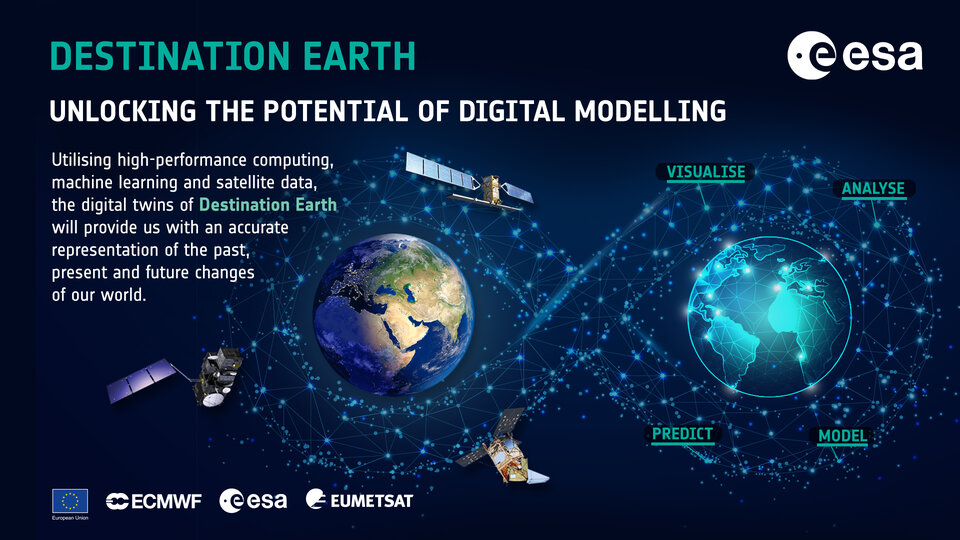
\includegraphics{training-materials/presentation/digital_twins.jpeg}

\hypertarget{digital-landscapes-for-sustainable-agri-food-systems}{%
\section{Digital landscapes for sustainable agri-food
systems}\label{digital-landscapes-for-sustainable-agri-food-systems}}

\begin{itemize}
\item
  We need to ensure our foundations are \textbf{solid}
\item
  Data is the backbone of these developments
\item
  But data without knowledge will not suffice
\item
  We are well placed to work at this interface
\end{itemize}

\hypertarget{lets-get-started}{%
\section{Let's get started}\label{lets-get-started}}

\begin{itemize}
\item
  The target for this week:
  \href{https://systems-agronomy.github.io/lcas/toolbox/show_report}{Sample
  report and workflow}
\item
  Our first line of code:
\end{itemize}

\begin{Shaded}
\begin{Highlighting}[]
\DecValTok{1} \SpecialCharTok{+} \DecValTok{1}
\end{Highlighting}
\end{Shaded}

\begin{verbatim}
[1] 2
\end{verbatim}

\hypertarget{housekeeping}{%
\section{Housekeeping}\label{housekeeping}}

\begin{enumerate}
\def\labelenumi{\arabic{enumi}.}
\tightlist
\item
  In the mornings we will have presentations + working with our
  examples.
\item
  In the afternoons, everyone will work on their own code.
\item
  Our focus will be on supporting in-person participants.
\item
  For online participants - please use the Google Space to discuss and
  help each other.
\item
  If you have questions in the room - please ask anytime.
\item
  Your feedback and suggestion are dearly needed.
\end{enumerate}

\begin{figure}

{\centering 
\includegraphics[width=3.11in,height=\textheight]{training-materials/presentation/housekeep.jpg}

}

\end{figure}

\hypertarget{the-workflow}{%
\section{The workflow}\label{the-workflow}}

\begin{itemize}
\tightlist
\item
  Once we completed the workflow we can automate
\item
  We can recycle our scripts for cleaning, plotting, and communicating
\end{itemize}

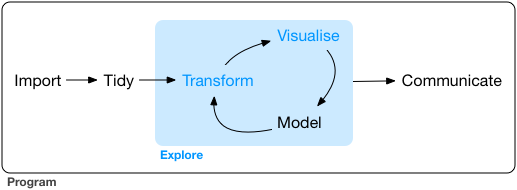
\includegraphics[width=2.08333in,height=\textheight]{training-materials/presentation/workflow.png}

\hypertarget{step-1---cleaning}{%
\section{Step 1 - Cleaning}\label{step-1---cleaning}}

\begin{itemize}
\tightlist
\item
  Time spend here - saves a lot of time later
\end{itemize}


\includegraphics[width=5.20833in,height=\textheight]{training-materials/presentation/meme1.jpeg}

\hypertarget{step-2---explore}{%
\section{Step 2 - Explore}\label{step-2---explore}}

\begin{itemize}
\tightlist
\item
  Understand distributions of key variables
\item
  Check for spatial variability
\item
  Run initial checks on key relationships
\end{itemize}


\includegraphics[width=3.125in,height=\textheight]{training-materials/presentation/explore.jpeg}

\hypertarget{step-3---advanced-analytics}{%
\section{Step 3 - Advanced
analytics}\label{step-3---advanced-analytics}}

\begin{itemize}
\tightlist
\item
  Build specific models - e.g.~yield prediction
\item
  Interrogate relationship inside the models
\item
  Run scenarios - e.g.~what happens to yield if we improve planting
  dates?
\item
  \href{https://www.statlearning.com/online-courses}{Free textbook and
  online course}
\end{itemize}

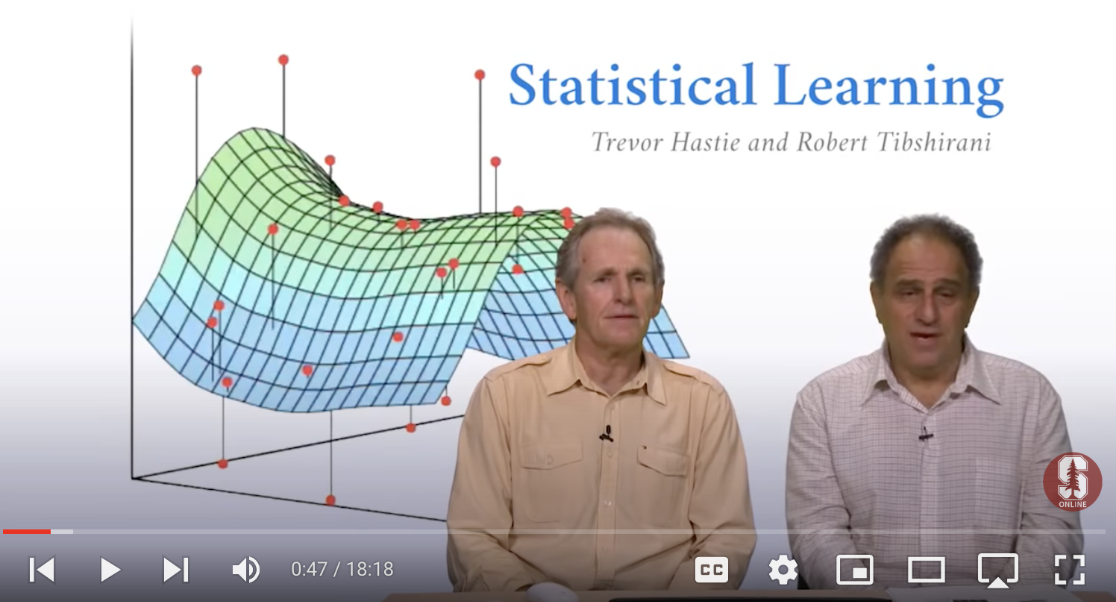
\includegraphics[width=4.16667in,height=\textheight]{training-materials/presentation/isl.png}

\hypertarget{step-4---communicate}{%
\section{Step 4 - Communicate}\label{step-4---communicate}}

\begin{itemize}
\tightlist
\item
  RStudio provides several handy functions for this.
\item
  Quarto documents are the current standard. You can generate websites,
  html documents, word reports and web applications.
\item
  This presentation was done in a Quarto document in RStudio.
\end{itemize}

\hypertarget{questions}{%
\section{Questions?}\label{questions}}

\hypertarget{some-basic-r-reminders}{%
\section{Some basic R reminders}\label{some-basic-r-reminders}}

\begin{itemize}
\tightlist
\item
  ``Es gibt nicht praktischerisch als eine gute Theorie''
\item
  ``There is nothing more practical than a good theory''
\item
  Source: German intellectual tradition, possibly Kant, Helmholtz.
\end{itemize}


\includegraphics[width=4.16667in,height=\textheight]{training-materials/presentation/kant.jpeg}

\hypertarget{this-is-all-you-need-really}{%
\section{This is all you need,
really}\label{this-is-all-you-need-really}}

\begin{itemize}
\tightlist
\item
  Atomic vectors (of different classes) - these hold values
\item
  And functions - `word' with (brackets) that run things.
\item
  Use c() to create vectors
\item
  Single numbers are vectors of length 1
\item
  Vectors can only have the same class - if mixed, they are converted to
  common class. Normally character.
\item
  R objects, unquoted names that we can assing things to
\item
  Assignment happens with: \textless-
\end{itemize}

\hypertarget{in-action}{%
\section{In action}\label{in-action}}

\begin{Shaded}
\begin{Highlighting}[]
\FunctionTok{is.vector}\NormalTok{(}\DecValTok{1}\NormalTok{) }\CommentTok{\# check whether this is a vector}
\end{Highlighting}
\end{Shaded}

\begin{verbatim}
[1] TRUE
\end{verbatim}

\begin{Shaded}
\begin{Highlighting}[]
\FunctionTok{class}\NormalTok{(}\DecValTok{1}\NormalTok{) }\CommentTok{\# check what class this vector is}
\end{Highlighting}
\end{Shaded}

\begin{verbatim}
[1] "numeric"
\end{verbatim}

\begin{Shaded}
\begin{Highlighting}[]
\FunctionTok{is.vector}\NormalTok{(}\StringTok{"Hello IRRI"}\NormalTok{)}
\end{Highlighting}
\end{Shaded}

\begin{verbatim}
[1] TRUE
\end{verbatim}

\begin{Shaded}
\begin{Highlighting}[]
\FunctionTok{class}\NormalTok{(}\StringTok{"Hello IRRI"}\NormalTok{)}
\end{Highlighting}
\end{Shaded}

\begin{verbatim}
[1] "character"
\end{verbatim}

\begin{Shaded}
\begin{Highlighting}[]
\FunctionTok{is.vector}\NormalTok{(}\FunctionTok{c}\NormalTok{(}\DecValTok{1}\NormalTok{,}\DecValTok{2}\NormalTok{))}
\end{Highlighting}
\end{Shaded}

\begin{verbatim}
[1] TRUE
\end{verbatim}

\begin{Shaded}
\begin{Highlighting}[]
\FunctionTok{c}\NormalTok{(}\StringTok{"HELLO IRRI"}\NormalTok{, }\DecValTok{1}\NormalTok{,}\DecValTok{2}\NormalTok{)}
\end{Highlighting}
\end{Shaded}

\begin{verbatim}
[1] "HELLO IRRI" "1"          "2"         
\end{verbatim}

\begin{Shaded}
\begin{Highlighting}[]
\FunctionTok{class}\NormalTok{(}\FunctionTok{c}\NormalTok{(}\StringTok{"HELLO IRRI"}\NormalTok{, }\DecValTok{1}\NormalTok{,}\DecValTok{2}\NormalTok{))}
\end{Highlighting}
\end{Shaded}

\begin{verbatim}
[1] "character"
\end{verbatim}

\begin{Shaded}
\begin{Highlighting}[]
\NormalTok{x }\OtherTok{\textless{}{-}} \FunctionTok{c}\NormalTok{(}\DecValTok{1}\NormalTok{,}\DecValTok{2}\NormalTok{,}\DecValTok{3}\NormalTok{) }
\FunctionTok{print}\NormalTok{(x)}
\end{Highlighting}
\end{Shaded}

\begin{verbatim}
[1] 1 2 3
\end{verbatim}

\hypertarget{everything-else}{%
\section{Everything else}\label{everything-else}}

\begin{itemize}
\item
  For our purposes, everything else are basically just construction of
  different vectors of varying levels of complexity.
\item
  We can also use attributes. These are things like the number of
  dimensions, or the names of columns or rows.
\item
  For example a data.frame is similar to an excel sheet. It just a
  collection of vectors (columns) of the same length, with a name for
  each column.
\end{itemize}

\hypertarget{in-action-1}{%
\section{In action}\label{in-action-1}}

\begin{Shaded}
\begin{Highlighting}[]
\NormalTok{farmer\_name }\OtherTok{\textless{}{-}} \FunctionTok{c}\NormalTok{(}\StringTok{"Hari"}\NormalTok{,}\StringTok{"Virender"}\NormalTok{,}\StringTok{"Anton"}\NormalTok{)}
\NormalTok{yield\_tha }\OtherTok{\textless{}{-}} \FunctionTok{c}\NormalTok{(}\FloatTok{10.3}\NormalTok{,}\FloatTok{5.3}\NormalTok{,}\FloatTok{2.3}\NormalTok{)}
\NormalTok{n\_rate }\OtherTok{\textless{}{-}} \FunctionTok{c}\NormalTok{(}\DecValTok{30}\NormalTok{,}\DecValTok{50}\NormalTok{,}\DecValTok{100}\NormalTok{)}

\NormalTok{survey }\OtherTok{\textless{}{-}} \FunctionTok{data.frame}\NormalTok{( }\CommentTok{\#here we ask to create a data frame. And assign it to survey}
  \AttributeTok{name =}\NormalTok{ farmer\_name,}
  \AttributeTok{yield =}\NormalTok{ yield\_tha, }\CommentTok{\# Here we create a column name "yield" and request yield\_tha as values}
  \AttributeTok{n =}\NormalTok{ n\_rate }\CommentTok{\# the same for n\_rate}
\NormalTok{)}

\NormalTok{survey }\CommentTok{\#ask to print the object survey}
\end{Highlighting}
\end{Shaded}

\begin{verbatim}
      name yield   n
1     Hari  10.3  30
2 Virender   5.3  50
3    Anton   2.3 100
\end{verbatim}

\begin{Shaded}
\begin{Highlighting}[]
\FunctionTok{dim}\NormalTok{(survey)}
\end{Highlighting}
\end{Shaded}

\begin{verbatim}
[1] 3 3
\end{verbatim}

\begin{Shaded}
\begin{Highlighting}[]
\FunctionTok{colnames}\NormalTok{(survey)}
\end{Highlighting}
\end{Shaded}

\begin{verbatim}
[1] "name"  "yield" "n"    
\end{verbatim}

\hypertarget{subsetting}{%
\section{Subsetting}\label{subsetting}}

\begin{itemize}
\tightlist
\item
  We can use the \textbf{{[}}index\_number\textbf{{]}} after an object
  to subset by stating the numbers that we want.
\item
  And index in R runs from 1 to n.
\item
  In data.frames we have two dimensions so we can use
  \textbf{{[}}row\_index,col\_index\textbf{{]}}. Blank space in one
  dimension means select all.
\end{itemize}

\hypertarget{in-action-2}{%
\section{In action}\label{in-action-2}}

\begin{Shaded}
\begin{Highlighting}[]
\NormalTok{farmer\_name[}\DecValTok{1}\NormalTok{] }\CommentTok{\# get the first farmner name }
\end{Highlighting}
\end{Shaded}

\begin{verbatim}
[1] "Hari"
\end{verbatim}

\begin{Shaded}
\begin{Highlighting}[]
\NormalTok{farmer\_name[}\DecValTok{2}\NormalTok{] }\CommentTok{\# get the second farmer name}
\end{Highlighting}
\end{Shaded}

\begin{verbatim}
[1] "Virender"
\end{verbatim}

\begin{Shaded}
\begin{Highlighting}[]
\NormalTok{farmer\_name[}\FunctionTok{c}\NormalTok{(}\DecValTok{1}\NormalTok{,}\DecValTok{2}\NormalTok{)] }\CommentTok{\# get both names}
\end{Highlighting}
\end{Shaded}

\begin{verbatim}
[1] "Hari"     "Virender"
\end{verbatim}

\begin{Shaded}
\begin{Highlighting}[]
\NormalTok{survey[}\DecValTok{1}\NormalTok{,}\DecValTok{1}\NormalTok{] }\CommentTok{\#subset the first entry in the first column}
\end{Highlighting}
\end{Shaded}

\begin{verbatim}
[1] "Hari"
\end{verbatim}

\begin{Shaded}
\begin{Highlighting}[]
\NormalTok{survey[}\DecValTok{1}\NormalTok{,] }\CommentTok{\#extract the entire first row  }
\end{Highlighting}
\end{Shaded}

\begin{verbatim}
  name yield  n
1 Hari  10.3 30
\end{verbatim}

\begin{Shaded}
\begin{Highlighting}[]
\NormalTok{survey[,}\DecValTok{3}\NormalTok{] }\CommentTok{\# extract the entire last column}
\end{Highlighting}
\end{Shaded}

\begin{verbatim}
[1]  30  50 100
\end{verbatim}

\begin{Shaded}
\begin{Highlighting}[]
\NormalTok{survey[,}\StringTok{"yield"}\NormalTok{] }\CommentTok{\#extract the column with the name "yield"}
\end{Highlighting}
\end{Shaded}

\begin{verbatim}
[1] 10.3  5.3  2.3
\end{verbatim}

\hypertarget{another-way-for-accessing-data-frame-columns}{%
\section{Another way for accessing data frame
columns}\label{another-way-for-accessing-data-frame-columns}}

\begin{itemize}
\tightlist
\item
  we can use the dollar sign (\$) with the name. This is easier to read.
\end{itemize}

\begin{Shaded}
\begin{Highlighting}[]
\NormalTok{survey}\SpecialCharTok{$}\NormalTok{name }\CommentTok{\#get the names column}
\end{Highlighting}
\end{Shaded}

\begin{verbatim}
[1] "Hari"     "Virender" "Anton"   
\end{verbatim}

\begin{Shaded}
\begin{Highlighting}[]
\NormalTok{survey}\SpecialCharTok{$}\NormalTok{n\_productivity }\OtherTok{\textless{}{-}}\NormalTok{ survey}\SpecialCharTok{$}\NormalTok{yield }\SpecialCharTok{/}\NormalTok{ survey}\SpecialCharTok{$}\NormalTok{n }\CommentTok{\# calculate the n producitivty}
\CommentTok{\#and assign to new column with name n\_productivity}

\NormalTok{survey}
\end{Highlighting}
\end{Shaded}

\begin{verbatim}
      name yield   n n_productivity
1     Hari  10.3  30      0.3433333
2 Virender   5.3  50      0.1060000
3    Anton   2.3 100      0.0230000
\end{verbatim}

\hypertarget{plotting}{%
\section{Plotting}\label{plotting}}

\begin{itemize}
\tightlist
\item
  we can use basic plotting and ggplot
\item
  for ggplot we need to load the ggplot2 library.
\item
  the `\textasciitilde{}' means `a function of'
\end{itemize}

\begin{Shaded}
\begin{Highlighting}[]
\FunctionTok{plot}\NormalTok{(survey}\SpecialCharTok{$}\NormalTok{yield}\SpecialCharTok{\textasciitilde{}}\NormalTok{survey}\SpecialCharTok{$}\NormalTok{n,}\AttributeTok{ylab =} \StringTok{"Yield"}\NormalTok{,}\AttributeTok{xlab=}\StringTok{"N rate"}\NormalTok{)}
\end{Highlighting}
\end{Shaded}

\begin{figure}[H]

{\centering 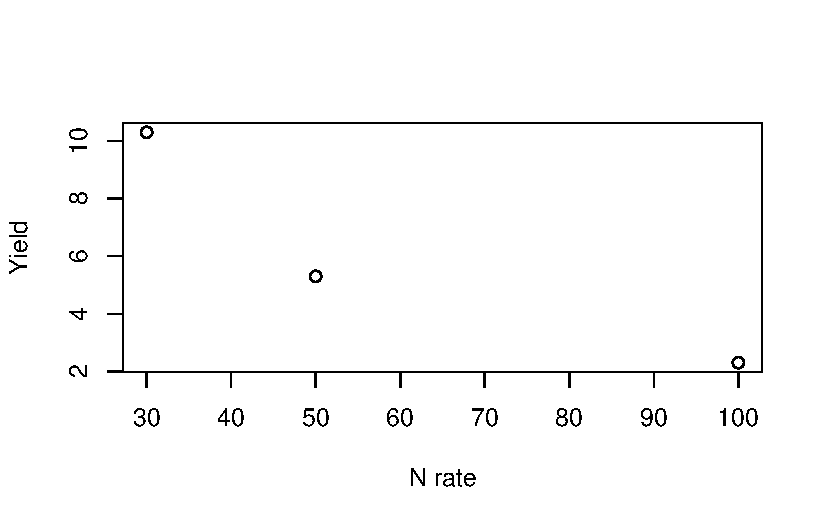
\includegraphics{training-materials/presentation/intro_files/figure-pdf/unnamed-chunk-6-1.pdf}

}

\end{figure}

\hypertarget{using-ggplot}{%
\section{using ggplot}\label{using-ggplot}}

\begin{Shaded}
\begin{Highlighting}[]
\FunctionTok{library}\NormalTok{(ggplot2)}

\FunctionTok{ggplot}\NormalTok{(}\AttributeTok{data =}\NormalTok{ survey)}\SpecialCharTok{+} \CommentTok{\#start a ggplot and use survey for data input}
  \FunctionTok{geom\_point}\NormalTok{(}\FunctionTok{aes}\NormalTok{(}\AttributeTok{x=}\NormalTok{n, }\AttributeTok{y=}\NormalTok{yield,}\AttributeTok{color=}\NormalTok{name))}\SpecialCharTok{+} \CommentTok{\#define aes(thetics), x axis, axis, color}
  \FunctionTok{theme\_classic}\NormalTok{()}\SpecialCharTok{+} \CommentTok{\#use classic theme for cleaner plot}
  \FunctionTok{scale\_x\_continuous}\NormalTok{(}\AttributeTok{name =} \StringTok{"N rate"}\NormalTok{) }\CommentTok{\#adjust the x axis. Name it N rate.}
\end{Highlighting}
\end{Shaded}

\begin{figure}[H]

{\centering 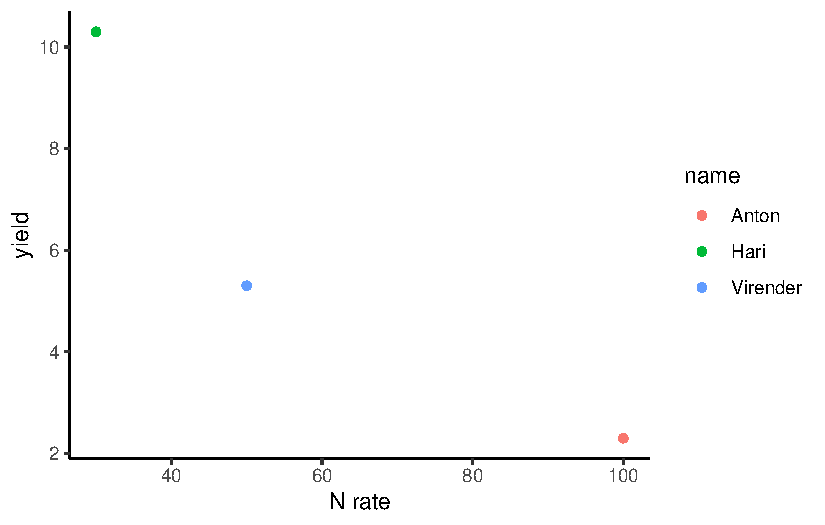
\includegraphics{training-materials/presentation/intro_files/figure-pdf/unnamed-chunk-7-1.pdf}

}

\end{figure}

\hypertarget{run-a-model}{%
\section{Run a model}\label{run-a-model}}

\begin{itemize}
\tightlist
\item
  run linear regression. Assign results to fit
\end{itemize}

\begin{Shaded}
\begin{Highlighting}[]
\NormalTok{fit }\OtherTok{\textless{}{-}} \FunctionTok{lm}\NormalTok{(}\AttributeTok{data =}\NormalTok{ survey, }\AttributeTok{formula =}\NormalTok{ yield}\SpecialCharTok{\textasciitilde{}}\NormalTok{n)}
\NormalTok{fit}
\end{Highlighting}
\end{Shaded}

\begin{verbatim}

Call:
lm(formula = yield ~ n, data = survey)

Coefficients:
(Intercept)            n  
    12.1974      -0.1038  
\end{verbatim}

\hypertarget{when-in-doubt-use-help-manuals---then-google}{%
\section{When in doubt, use help manuals - then
google}\label{when-in-doubt-use-help-manuals---then-google}}

\begin{itemize}
\tightlist
\item
  can use ? to get the help page of the function.
\item
  often things can be clarified by reading these carefully.
\item
  Googling can take quite some time - if you don't find the solution to
  your problem after 10min. Just send us a quick message.
\end{itemize}

\begin{Shaded}
\begin{Highlighting}[]
\NormalTok{?mean}
\end{Highlighting}
\end{Shaded}

\hypertarget{questions-1}{%
\section{Questions?}\label{questions-1}}

Off to the real fun! And using your own examples.

You can download all of the course materials incl.~this deck from this
github repo: \url{https://github.com/AntonUrfels/data-works}. You can
also look at them at the link of the corresponding website
\url{https://antonurfels.github.io/data-works/}.

\bookmarksetup{startatroot}

\hypertarget{references}{%
\chapter*{References}\label{references}}
\addcontentsline{toc}{chapter}{References}

\markboth{References}{References}

\hypertarget{refs}{}
\begin{CSLReferences}{0}{0}
\end{CSLReferences}



\end{document}
